
\documentclass[acmtog]{acmart}

\usepackage{graphicx}
\usepackage{subcaption}
\usepackage{hyperref}

\graphicspath{ {./images/} }

\AtBeginDocument{%
	\providecommand\BibTeX{{%
			\normalfont B\kern-0.5em{\scshape i\kern-0.25em b}\kern-0.8em\TeX}}}

\setcopyright{acmcopyright}
\copyrightyear{2023}
\acmYear{2023}
\acmDOI{XXXXXXX.XXXXXXX}

\begin{document}
	\title{Land Use Classification Project Proposal}
	
	\author{Thai La}
	\email{vtl932@usask.ca}
	\orcid{1234-5678-9012}
	\affiliation{%
		\institution{University of Saskatchewan}
		\streetaddress{105 Administration Pl}
		\city{Saskatoon}
		\state{Saskatchewan}
		\country{Canada}
		\postcode{S7N 5A2}
	}

	\keywords{Satellite, Image, Classification, LandUse, GeoSpatial}
	
	\maketitle
	
	\section{Introduction}
	This project aims to incorporate machine learning, deep learning and image processing techniques (if necessary) to classify land use within an image. The \href{https://git.cs.usask.ca/vtl932/cmpt318_course_project}{GitLab project repository} is the place where the project will live and the \href{https://www.kaggle.com/datasets/apollo2506/eurosat-dataset?select=EuroSAT}{Kaggle Dataset} is the source of the data.
	
	\section{Proposal}
	\label{sec:ProposalObjective}
	The objective of this data set:\\
	\begin{enumerate}
		\item Correctly identify the land use for each image in the image set.
	\end{enumerate}
	There are 10 total categories for land uses: AnnualCrop, Forest, HerbaceousVegetation, Highway, Industrial, Pasture, PermanentCrop, Residential, River, and Sealake.\\
	This dataset is within the scope of a multi-classification problem since there are 10 categories of land use which an image can be classified into.\\
	The license under which the dataset is released is \href[]{https://creativecommons.org/publicdomain/zero/1.0/}{CC0: Public Domain}.
	
	\subsection{Motivation}	
	The rationale behind choosing this dataset is to learn image classification using machine learning and deep learning techniques. The domain of computer vision and image processing is also a topic of intrigue and interest to me, which was what initially drove me to select this dataset.
	
	\subsection{Importance}
	This task will be challenging to solve due to the involvement of computer vision and image processing techniques. Utilizing and understanding such techniques will require exploration of these subjects and being able to integrate those techniques into the primary objective of this project, which is the classification of land use for an image.\\
	\\
	This project/task holds important significance because of its potential to identify potential disturbances to wildlife habitats caused by anthropogenic activities, notably urbanization and industrialization. Identifying such disturbances will allow either a relocation of the impacted species to a different habitat or reforming certain areas of urbanization and industrialization as natural protected areas.\\
	Additionally, land use classification can play a crucial role in identifying optimal land utilization for vacant or unused areas, which can further safeguard the natural wildlife habitats from urbanization or industrialization.
	
	\subsection{Analysis}
	This task will be situated within the domain of machine learning, and potentially involving deep learning techniques as well as computer vision and image processing techniques.\\
	The input data for the training, testing and validation dataset consists of 64x64 RGB images with a Ground Sampling Distance of 10m, with each image representing a distinct land use category. The desired output corresponds to the classification label for each land use category.\\
	The metric used to gauge performance of the model will be the accuracy metric and the loss metric. That is, the higher the accuracy and lower the loss, the better the model is.
	\subsubsection{Approaches:}
	\begin{itemize}
		\item One clear approach is to use Convultional Neural Networks (CNNs) to identify land use of an image. However, this approach can only identify one land use for the entire image, which will satisfy the primary objective of this project. Please note that the original objective posted by Kaggle is to identify the top 2 uses of land in an image. Approaching the problem from Kaggle's objective will require some sort of segmentation techniques and/or Region-based Convolutional Neural Networks (RCNNs). To simplify the task, this project will focus solely on correctly identifying the land use of one image (please refer to the \hyperref[sec:ProposalObjective]{proposal objective}).
		
		\item Another approach is to make use of an algorithm specifically designed for land use classification. To explore this approach, I plan on looking at some research papers that focuses on land use classification. This approach is only secondary and is meant to provide me with insights into tackling the problem.
		
	\end{itemize}
	Ultimately, I plan on implementing the described first approach, which is to use CNNs.
	
	\section{Conclusion}
	In conclusion, the goal of this project is to correctly identify land use for each 64x64 RGB image in the image dataset. The metric to measure performance will be accuracy and loss function.
	

	\begin{minipage}{\textwidth}
		\begin{subfigure}[h]{0.5\linewidth}
			\centering
			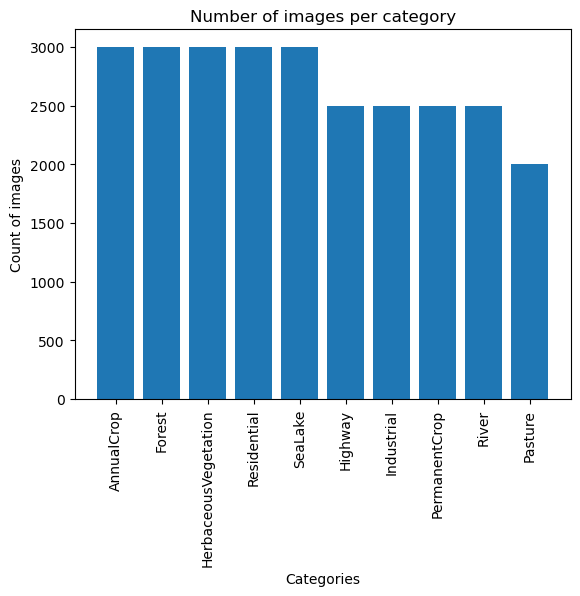
\includegraphics[scale=0.6]{Fig1.png} \\
			Figure 1. Dataset Figure - Number of images per category label
		\end{subfigure}
		\begin{subfigure}[h]{0.5\linewidth}
			\centering
			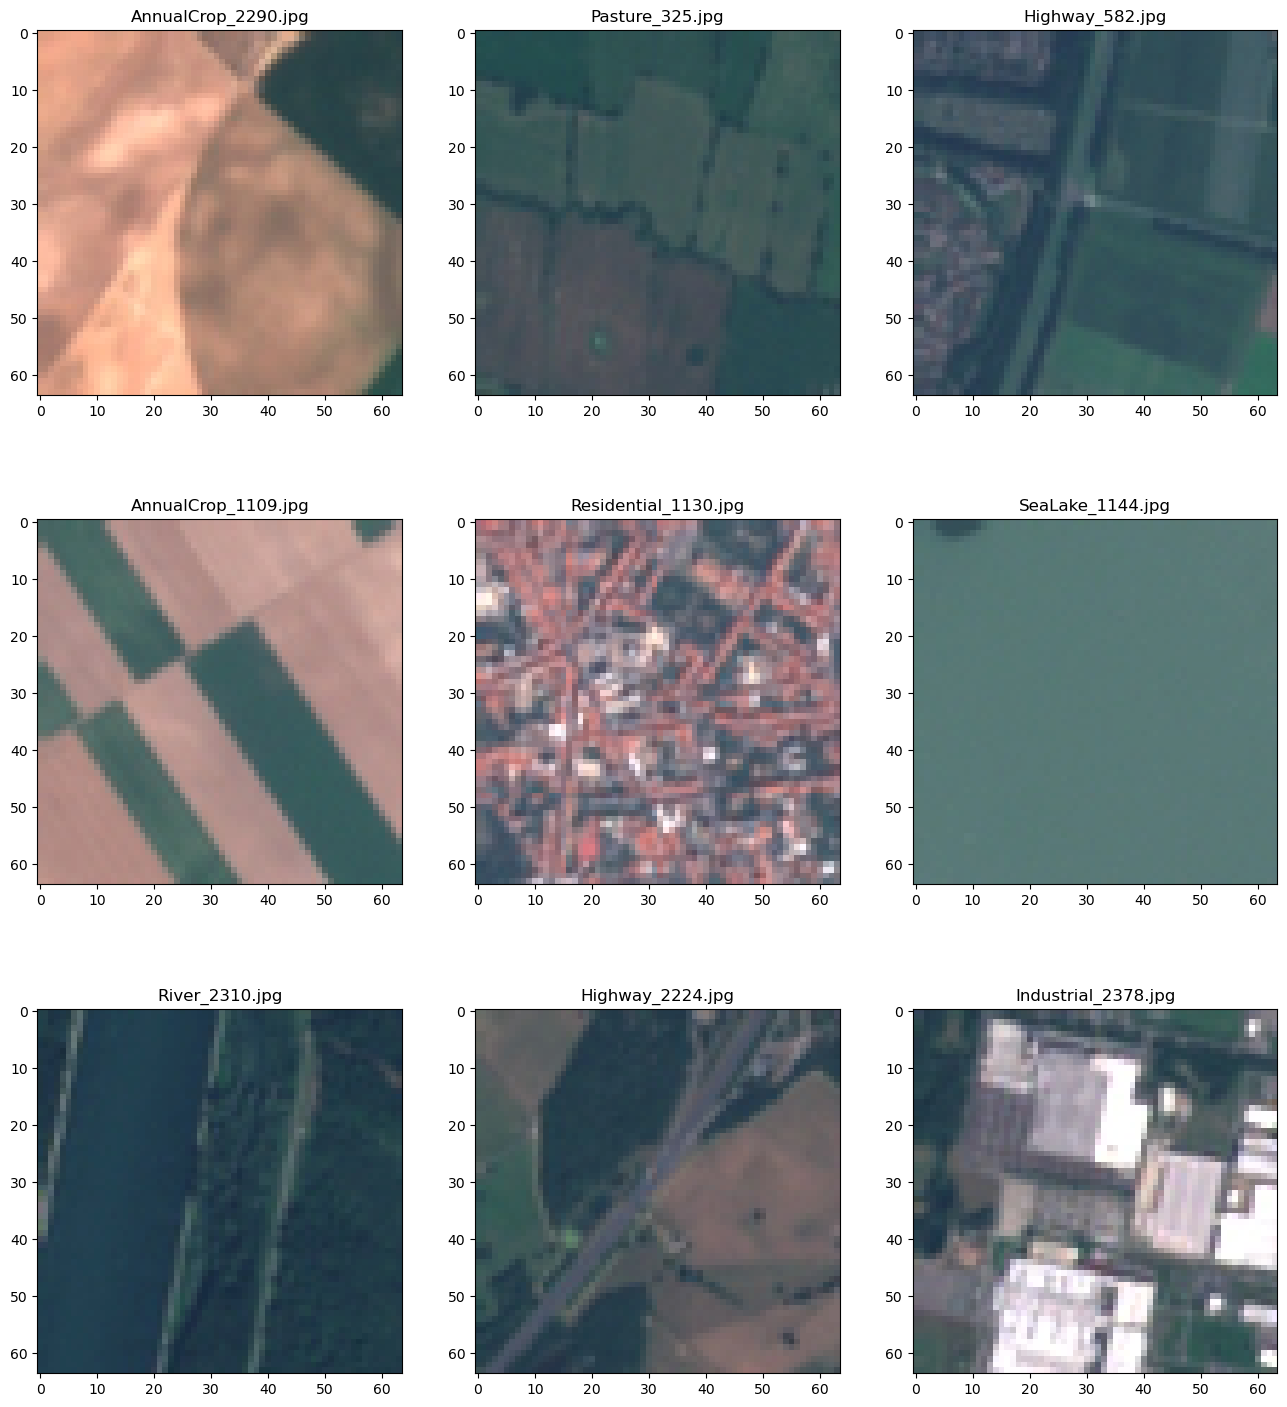
\includegraphics[scale=0.3]{Fig2.png} \\
			Figure 2. Data Sample figure - Input data
		\end{subfigure}\vspace*{35}
		\begin{subfigure}[h]{\linewidth}
			\centering
			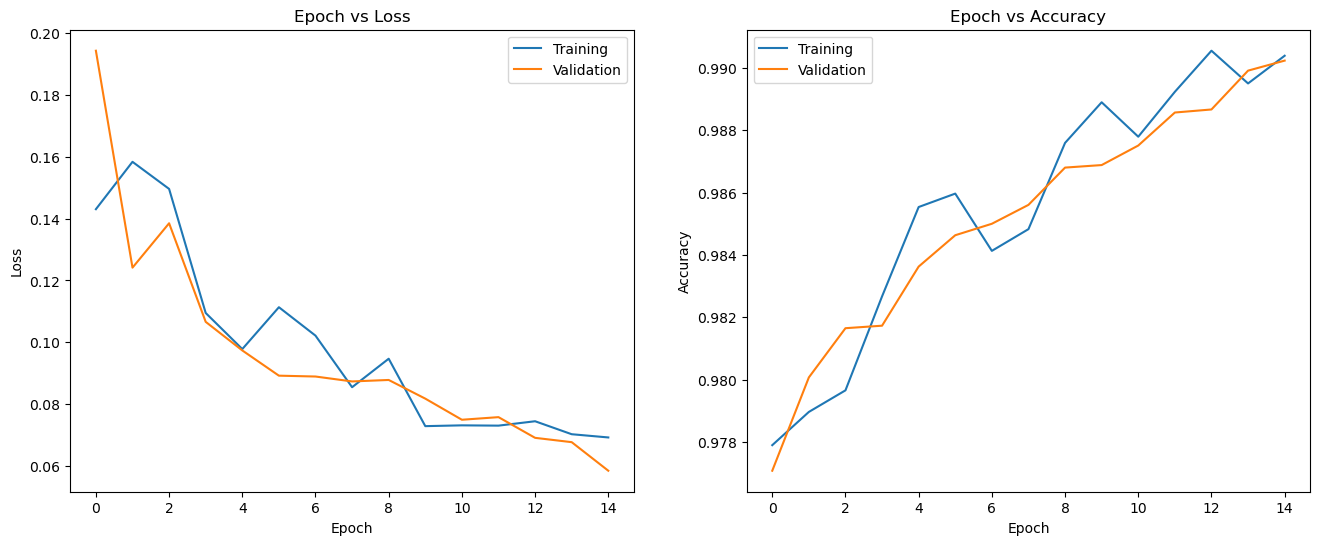
\includegraphics[scale=0.5]{Fig3.png} \\
			Figure 3. Proposed Results figure - Accuracy and Loss measured at each Epoch
		\end{subfigure}
	\end{minipage}
		
\end{document}
\endinput
